%                                                                 aa.dem
% AA vers. 9.1, LaTeX class for Astronomy & Astrophysics
% demonstration file
%                                                       (c) EDP Sciences
%-----------------------------------------------------------------------
%
%\documentclass[referee]{aa} % for a referee version
%\documentclass[onecolumn]{aa} % for a paper on 1 column  
%\documentclass[longauth]{aa} % for the long lists of affiliations 
%\documentclass[letter]{aa} % for the letters 
%\documentclass[bibyear]{aa} % if the references are not structured 
%                              according to the author-year natbib style

%
\documentclass{aa}  

%
\usepackage{graphicx}
%%%%%%%%%%%%%%%%%%%%%%%%%%%%%%%%%%%%%%%%
\usepackage{txfonts}
%%%%%%%%%%%%%%%%%%%%%%%%%%%%%%%%%%%%%%%%
%\usepackage[options]{hyperref}
% To add links in your PDF file, use the package "hyperref"
% with options according to your LaTeX or PDFLaTeX drivers.
%
\begin{document} 


   \title{Simulating the Universe from the Cosmic Microwave Background to Today}

   \subtitle{}

   \author{A. Martins
          \inst{1}
          }

   \institute{Institute of Theoretical Astrophysics, University of Oslo,
              Sem Sælands vei 13, 0371 Oslo\\
              \email{a.i.s.martins@astro.uio.no}
             }

   \date{}

% \abstract{}{}{}{}{} 
% 5 {} token are mandatory
 
  \abstract
  % context heading (optional)
  % {} leave it empty if necessary  
   {}
  % aims heading (mandatory)
   {}
  % methods heading (mandatory)
   {}
  % results heading (mandatory)
   {}
  % conclusions heading (optional), leave it empty if necessary 
   {}

   \keywords{
               }

   \maketitle
%
%-------------------------------------------------------------------

\section{Introduction}

\subsection{Background Cosmology}

\section{Theoretical background}

\subsection{Background Cosmology}

We start by assuming that, at large scales, matter is homogeneous and isotropic. The mathematical formulation of this, i.e. the metric that describes the geometry of the Universe at large scales is given by the Friedmann–Lemaître–Robertson–Walker (FRLW) metric:
\begin{equation}
ds^2 = -dt^2 + a^2(t)(dx^2 + dy^2 + dz^2),
\end{equation}
where $a(t)$ is the scale factor of the Universe, a measure for the rate of its expansion.

We are interested in learning about the densities of the different components of the Universe at different points in time, from the Cosmic Microwave Background until the present day. The $\Lambda$CDM model assumes that the Universe is composed of matter (baryons\footnote{Baryons in this context refers to all "normal" matter, i.e. quarks, leptons (not including neutrinos for our purposes) and combinations of them.} and cold, dark matter), radiation (photons and neutrinos) and dark energy. Another important notion for our model is that of curvature, which we already implicitly assumed to be 0 in the above equation, i.e. we are assuming a flat Universe. These components come together in the Friedman equation, which relates their density evolution to the expansion of the Universe:
\begin{equation}
H(a) = H_0 \sqrt{\Omega_{M0}a^{-3} + \Omega_{R0}a^{-4} + \Omega_{k 0} a^{-2} + \Omega_{\Lambda 0}},
\end{equation}
where $H(a)$ is the so-called Hubble parameter and $H_0$ is the Hubble constant, measured experimentally today to be around 68.3 km s$^{-1}$ Mpc$^{-1}$ \citep{Kozmanyan_2019}. Each $\Omega_{i0}$ represents the density of one of the above-mentioned components in the present day, now explicitly including curvature $k$, and $\Omega_{M0} = \Omega_{b0} + \Omega_\text{CDM0}, \Omega_{R0} = \Omega_{\gamma0} + \Omega_{\nu0}$. The densities for photons and neutrinos today are given by
\begin{align}
\Omega_{\gamma 0} &= 2\cdot \frac{\pi^2}{30} \frac{(k_bT_{\rm CMB 0})^4}{\hbar^3 c^5} \cdot \frac{8\pi G}{3H_0^2},\\
\Omega_{\nu 0} &= N_{\rm eff}\cdot \frac{7}{8}\cdot \left(\frac{4}{11}\right)^{4/3}\Omega_{\gamma 0},
\end{align}
whereas the densities for 

We can get the component densities for different scale factors from
\begin{align}
\Omega_{k}(a) &= \frac{\Omega_{k0}}{a^2H(a)^2/H_0^2}\\
\Omega_{\rm CDM}(a) &= \frac{\Omega_{\rm CDM 0}}{a^3H(a)^2/H_0^2} \\
\Omega_b(a) &= \frac{\Omega_{b 0}}{a^3H(a)^2/H_0^2} \\
\Omega_\gamma(a) &= \frac{\Omega_{\gamma 0}}{a^4H(a)^2/H_0^2} \\
\Omega_{\nu}(a) &= \frac{\Omega_{\nu 0}}{a^4H(a)^2/H_0^2} \\
\Omega_{\Lambda}(a) &= \frac{\Omega_{\Lambda 0}}{H(a)^2/H_0^2}.
\end{align}



\section{Implementation, numerical methods and tests}

\subsection{Background Cosmology}

\section{Results}

\subsection{Background Cosmology}

\begin{figure}[ht]
\centering
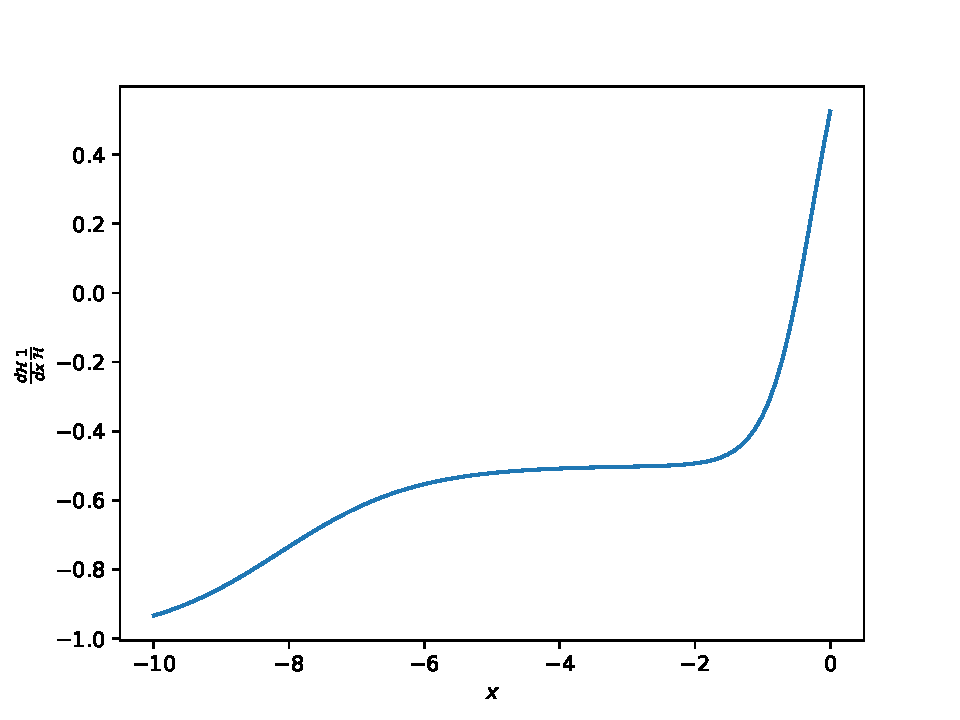
\includegraphics[width=\hsize]{figures/dHpdx_over_Hp.pdf}
  \caption{}
     \label{}
\end{figure}

\begin{figure}[ht]
\centering
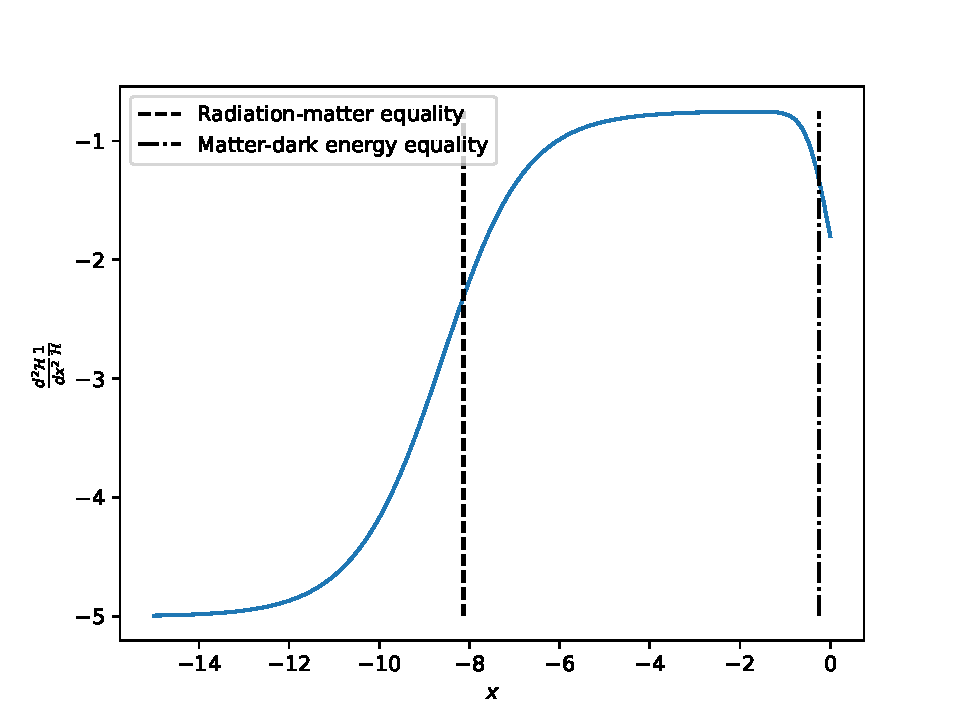
\includegraphics[width=\hsize]{figures/ddHpddx_over_Hp.pdf}
  \caption{}
     \label{}
\end{figure}

\begin{figure}[ht]
\centering
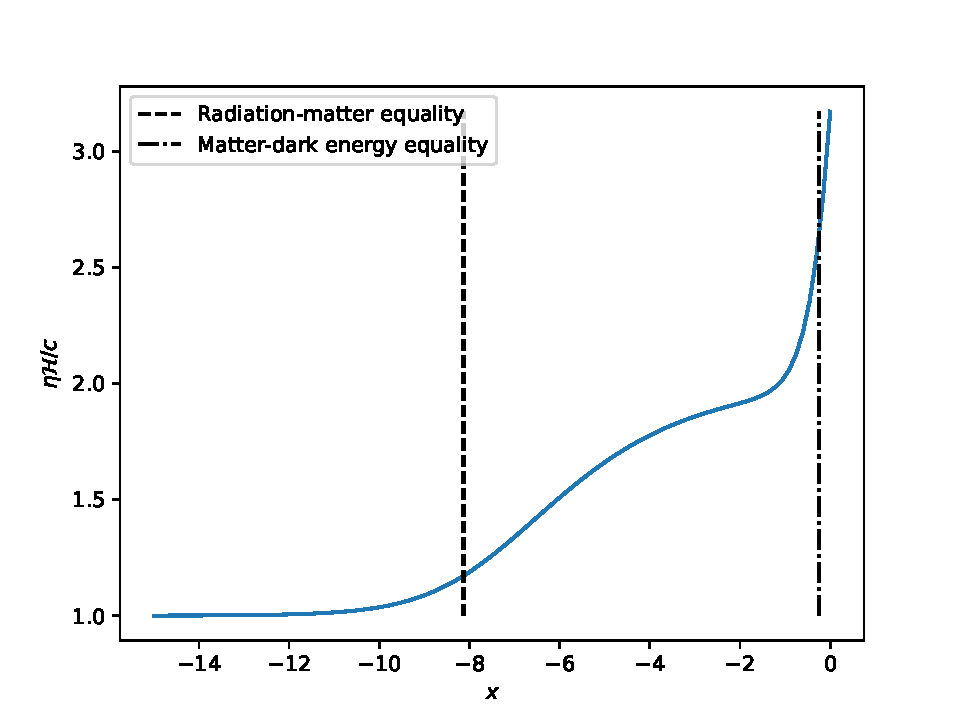
\includegraphics[width=\hsize]{figures/etaHp_over_c.pdf}
  \caption{}
     \label{}
\end{figure}

\begin{figure}[ht]
\centering
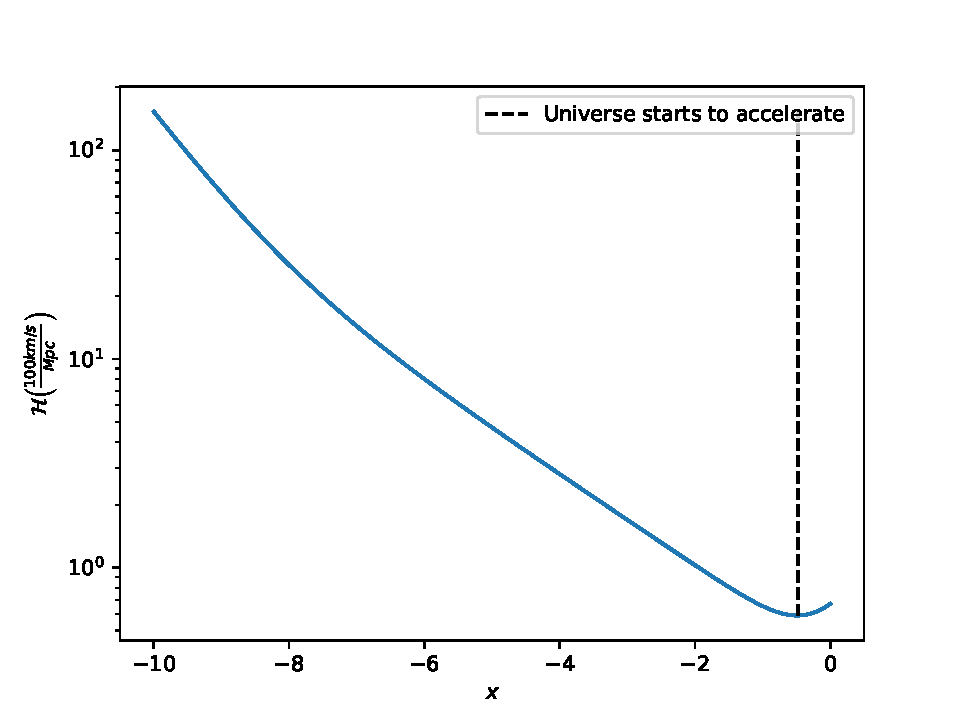
\includegraphics[width=\hsize]{figures/Hp.pdf}
  \caption{}
     \label{}
\end{figure}

\begin{figure}[ht]
\centering
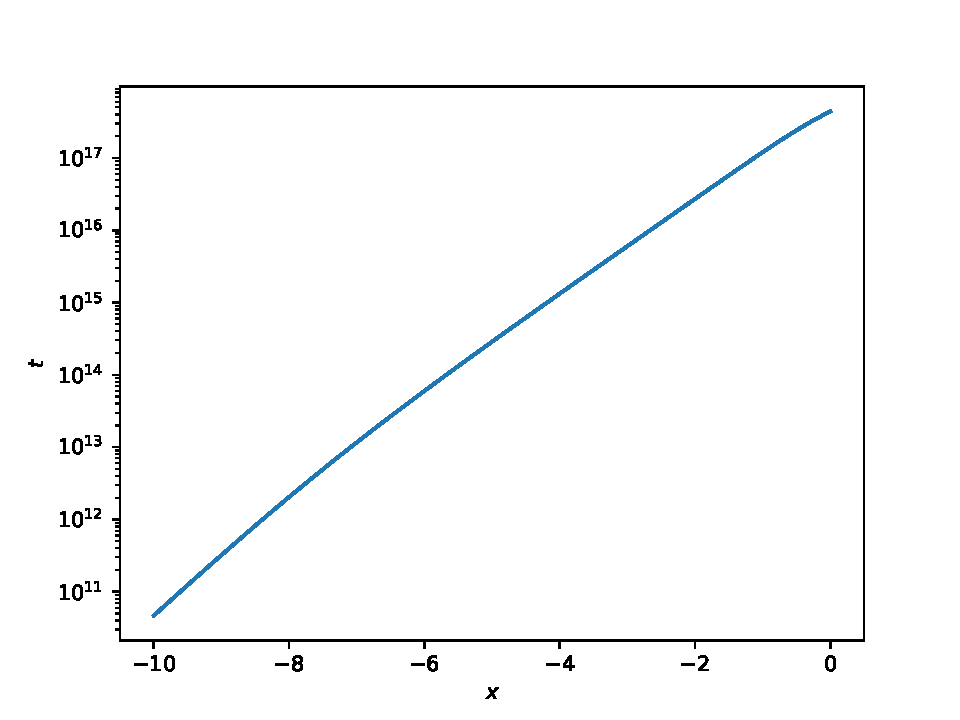
\includegraphics[width=\hsize]{figures/t.pdf}
  \caption{}
     \label{}
\end{figure}

\begin{figure}[ht]
\centering
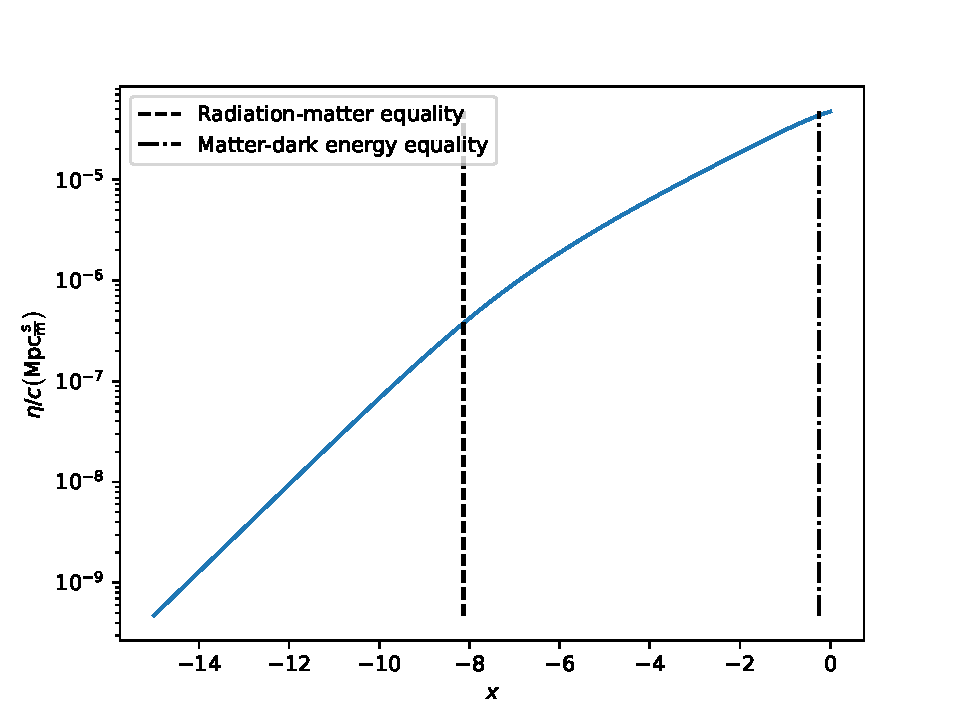
\includegraphics[width=\hsize]{figures/eta_over_c.pdf}
  \caption{}
     \label{}
\end{figure}

\begin{figure}[ht]
\centering
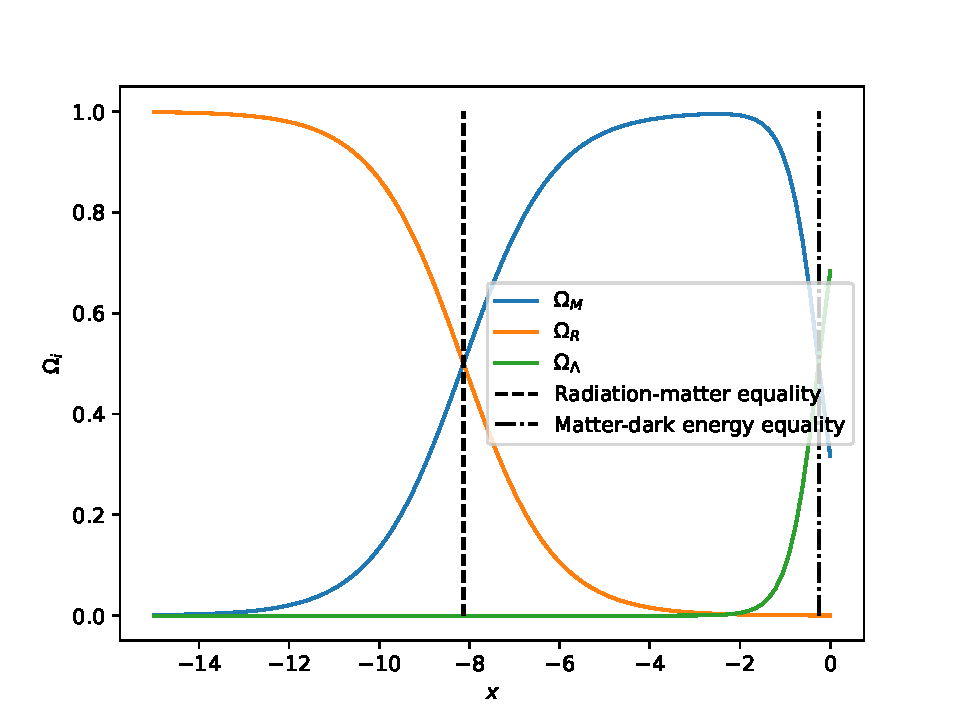
\includegraphics[width=\hsize]{figures/Omegas.pdf}
  \caption{}
     \label{}
\end{figure}

\begin{figure}[ht]
\centering
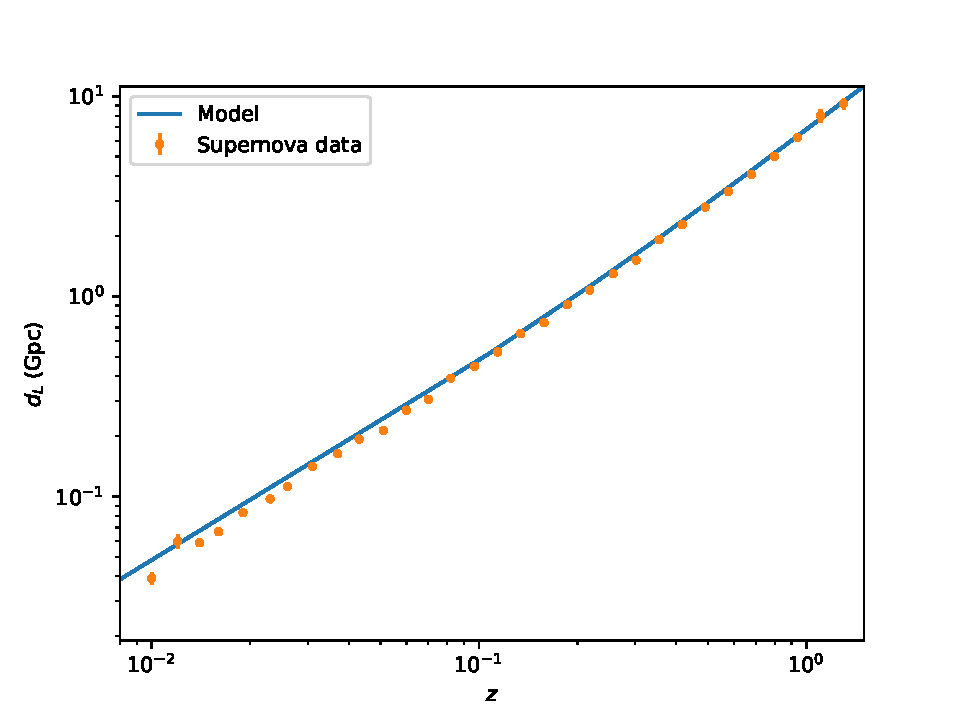
\includegraphics[width=\hsize]{figures/dL.pdf}
  \caption{}
     \label{}
\end{figure}

\begin{figure}[ht]
\centering
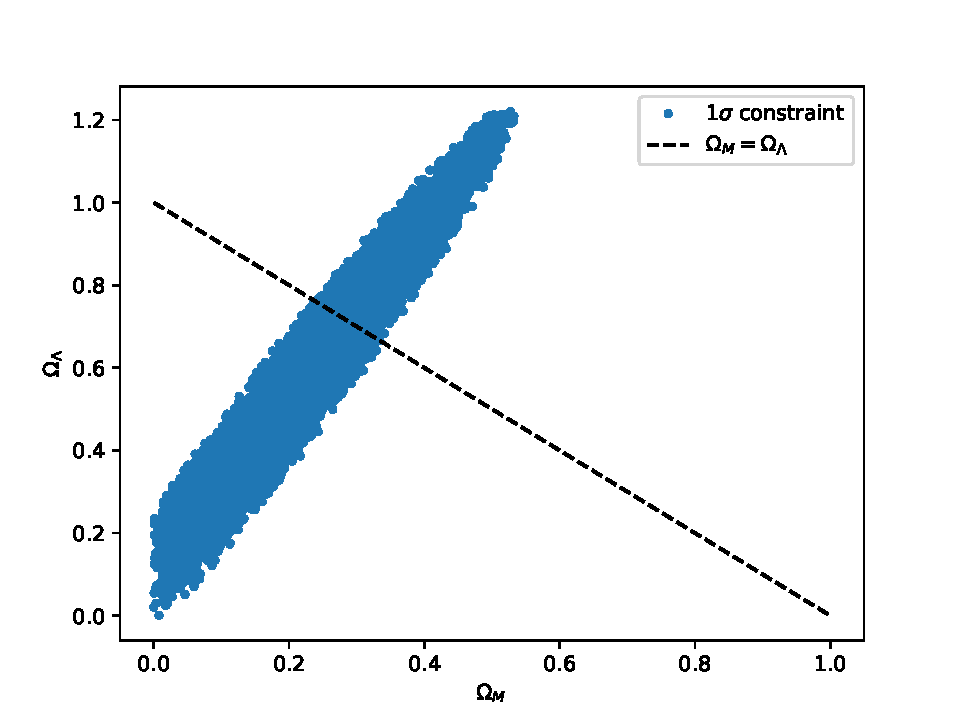
\includegraphics[width=\hsize]{figures/fitting.pdf}
  \caption{}
     \label{}
\end{figure}

\begin{figure}[ht]
\centering
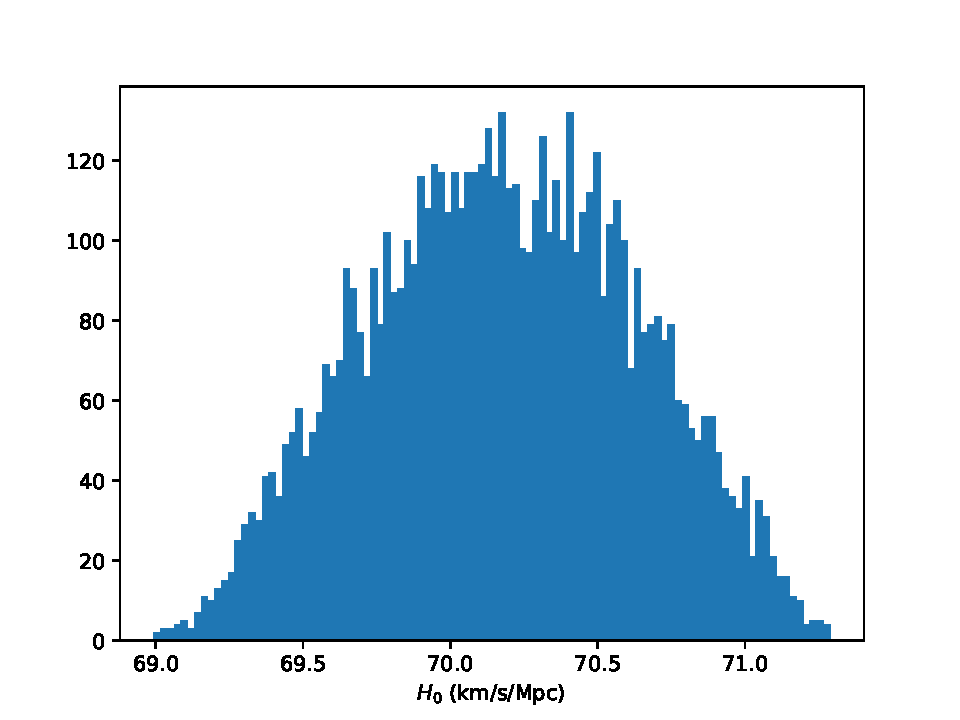
\includegraphics[width=\hsize]{figures/histogram.pdf}
  \caption{}
     \label{}
\end{figure}

%                                             Two column Table 
%-------------------------------------------------------------
%
\begin{table*}[ht]
\caption{Nonlinear Model Results}             
\label{table:1}      
\centering          
\begin{tabular}{l l l l}     % 7 columns 
\hline\hline       
                      % To combine 4 columns into a single one 
& Logarithm of scale factor $x$      & Redshift $z$     & Cosmic time $t$ (Gyr)\\ 
\hline                    
Radiation-Matter Equality   & -8.1319  & 3400.3  & 5.1029 $\times 10^{-5}$ \\
Matter-Dark Energy Equality & -0.25582 & 0.29152 & 10.371                 \\
$\ddot a = 0$               & -0.47941 & 0.61513 & 7.8234\\ 
\hline                  
\end{tabular}
\end{table*}

The conformal time of today ($a = 1 \Rightarrow x = 0$) is 14.192 Gpc.

\section{Conclusions}

\subsection{Background Cosmology}

\begin{acknowledgements}

\end{acknowledgements}

% WARNING
%-------------------------------------------------------------------
% Please note that we have included the references to the file aa.dem in
% order to compile it, but we ask you to:
%
% - use BibTeX with the regular commands:
%   \bibliographystyle{aa} % style aa.bst
%   \bibliography{Yourfile} % your references Yourfile.bib
%
% - join the .bib files when you upload your source files
%-------------------------------------------------------------------

\bibliographystyle{aa}
\bibliography{report/references}

\end{document}
